\subsection{Phylogeny mostly gets it right, but bad seeds spread}\label{sec:dd-iba}
\textbf{Claim.} IBA is the best-performing inferred evidence (\accIBA\% accepted, \rejIBA\% rejected),
because PAINT curators place functions at tree nodes after reading every descendant's evidence.
Its failures are structured: node placed too deep, neo-functionalised subfamilies, pseudoenzymes,
and above all a wrong \emph{seed}: one experimental annotation on one protein becomes an IBA on
every descendant.
\textbf{Corpus.} \nPropRows{} annotations on \nPropGenes{} genes carry a structured propagation review
recording why a transferred annotation holds or fails (Fig.~\ref{fig:propagation}). \pctPropNoFailure\% show
no failure; \pctPropScoping\% are term-scoping problems (the transfer is sound but the term is too broad or
too narrow); \pctPropBad\% are bad propagation and \pctPropSource\% trace to a weak, wrong or stale source.
No-failure rates differ sharply by code: IBA \pctPropNoFailureIBA\%, ISO \pctPropNoFailureISO\%.
Granularity mismatch and role conflation are the most frequently named failure modes.
\begin{figure}[t]\centering
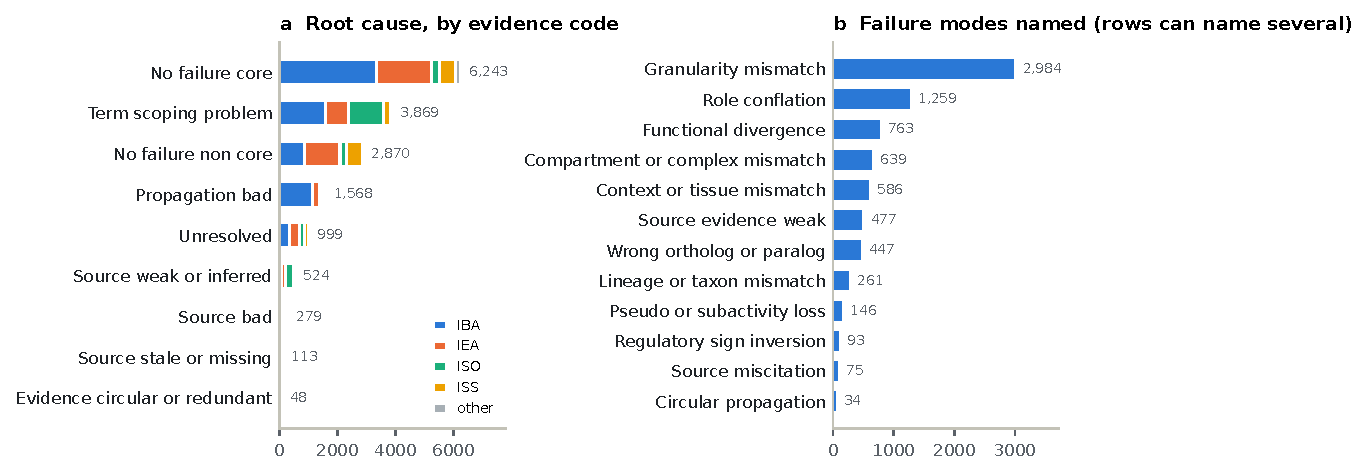
\includegraphics[width=\linewidth]{figures/propagation.pdf}
\caption{Structured propagation reviews of transferred annotations. (a) Root cause assigned, split by
evidence code. (b) Failure modes named; one row may name several.}
\label{fig:propagation}
\end{figure}
\textbf{Projects.} \proj{IBA\_REVIEW.md}: 16 failure patterns, 79 worked cases; IBA too conservative
for core MF in human as well. \proj{PANTHER\_IBA\_REVIEW.md}: all 160 IBAs on 41 \textit{S.\ pombe}
genes rebuilt from source node; 148 kept. \proj{PSEUDOCAP.md}: of 109 \textit{P.\ aeruginosa} proteins
that are the \emph{sole} seed of a PAINT node term, 21 carry a wrong or indirect seed (catalase activity
on a heme exporter, a mistyped GO id on pilU, signal transduction on a signal synthase).
\proj{CACAO.md}: student community annotations (\nCACAO{} rows here, \accCACAO\% accepted).
\proj{TRANSCRIPTION\_FACTORS.md}: netrins carrying dbTF activity from a POU-seeded node.
\proj{CONSERVED\_FUNCTION\_RECOVERY.md}: nearly every flagellar/T3SS export ATPase (FliI/SctN) in
UniProt annotated as F-type ATP synthase via PAINT, TreeGrafter, InterPro2GO and GO logical inference.
Where a transfer stands or falls on a residue, reviews record a checkable residue claim
(\S\ref{sec:seqchecks}); \nResRetained{} of \nResClaims{} claims are \emph{retained} sites, which refute a
proposed loss rather than confirm one.
\textbf{Message.} Argue with the node and the seed, not with donor count; one fix at the seed or
node corrects every descendant.
